
%%%%%%%%%%%%%%%%%%%%%%%%%%%%%%%%%%%%%%%%%%%%%%%%%%%%%%%%%%%%%%%%%%%%%%%%%%%%%%%%
\section{Introduction}
Faced with the nuclear spent fuel disposal siting challenge, creative solutions 
are necessary. This work proposes and evaluates a strategy that leverages the 
remaining resources inherent in a shutdown nuclear reactor site.

% add two sentences  about  current and projected nuclear plant shutdowns.

% add sentences regarding the DOE decision to pursue consent based siting.

% explain that this work compares the base case with the proposal
% note the metrics on which these two cases are being compared.

\subsection{Motivation}
The proposed integrated siting strategy takes advantage of three technical 
benefits of borehole repository designs: modularity, broad geological 
suitability, and footprint efficiency. Modularity enables regional repositories 
to scale in size according to the local spent fuel burden. 
Additionally, the necessary geological characteristics required for borehole 
disposal, crystalline basement rocks at $2,000 m - 5,000 m$ deep, are relatively 
common in stable continental regions \cite{arnold_research_2012}. Finally, the 
surface footprint requirements of a borehole repository are comparable to the 
available footprint of a nuclear power reactor site, with only $30 km^2$ 
required for the total \gls{SNF} amount proposed for Yucca Mountain 
\cite{brady_deep_2009}.

Integrated siting also has potential economic benefits. One 
significant cost inherent to borehole repository concepts is the repacking of 
spent fuel assemblies into smaller-diameter waste canisters. However, siting a 
repository at a non-operating power plant facility, especially one with a 
dry-cask storage site, will take advantage of already existing infrastructure 
and local human talent for spent fuel handling and packaging. Many candidate 
non-operating reactor sites, such as those mapped in Figure \ref{fig:shutdown} 
may be appropriate for integrated siting if they are located above crystalline 
basement formations and include dry cask packaging facilities.


Preliminary work \cite{waleed_regional_2015} indicates integrated siting is 
appealing to many stakeholder groups. For example, a consent-based approval 
process may be feasible because communities local to power plants may be uniquely 
receptive to the incentives of hosting a repository.  

%%%%%%%%%%%%%%%%%%%%%%%%%%%%%%%%%%%%%%%%%%%%%%%%%%%%%%%%%%%%%%%%%%%%%%%%%%%%%%%

\section{Methodology}

This work will evaluate the potential impacts of integrated siting from the 
perspective of 5 stakeholders:
\begin{itemize}
        \item the federal government,
        \item the state government,
        \item the local government,
        \item the local community,
        \item and the owner of the non-operating plant.
\end{itemize}


Preliminary work \cite{waleed_regional_2015} suggests that integrated siting 
will reduce costs, construction, time (both for construction and licensing), 
transportation distances, and resistence from the local community.  The present 
work will compare the proposal along these axes to a base case: a standalone 
borehole repository at a similar location to that of Yucca Mountain.  
Quantification of those stakeholder benefits will be undertaken for two 
different regions of the US in addition to the base case.  

Unique parameters are quantified using simple calculations from easily accessible
data. The goal of this paper is to quantify different metrics in numbers in order
to clarify siting methodology.

\begin{figure}[!h] 
  \centering
  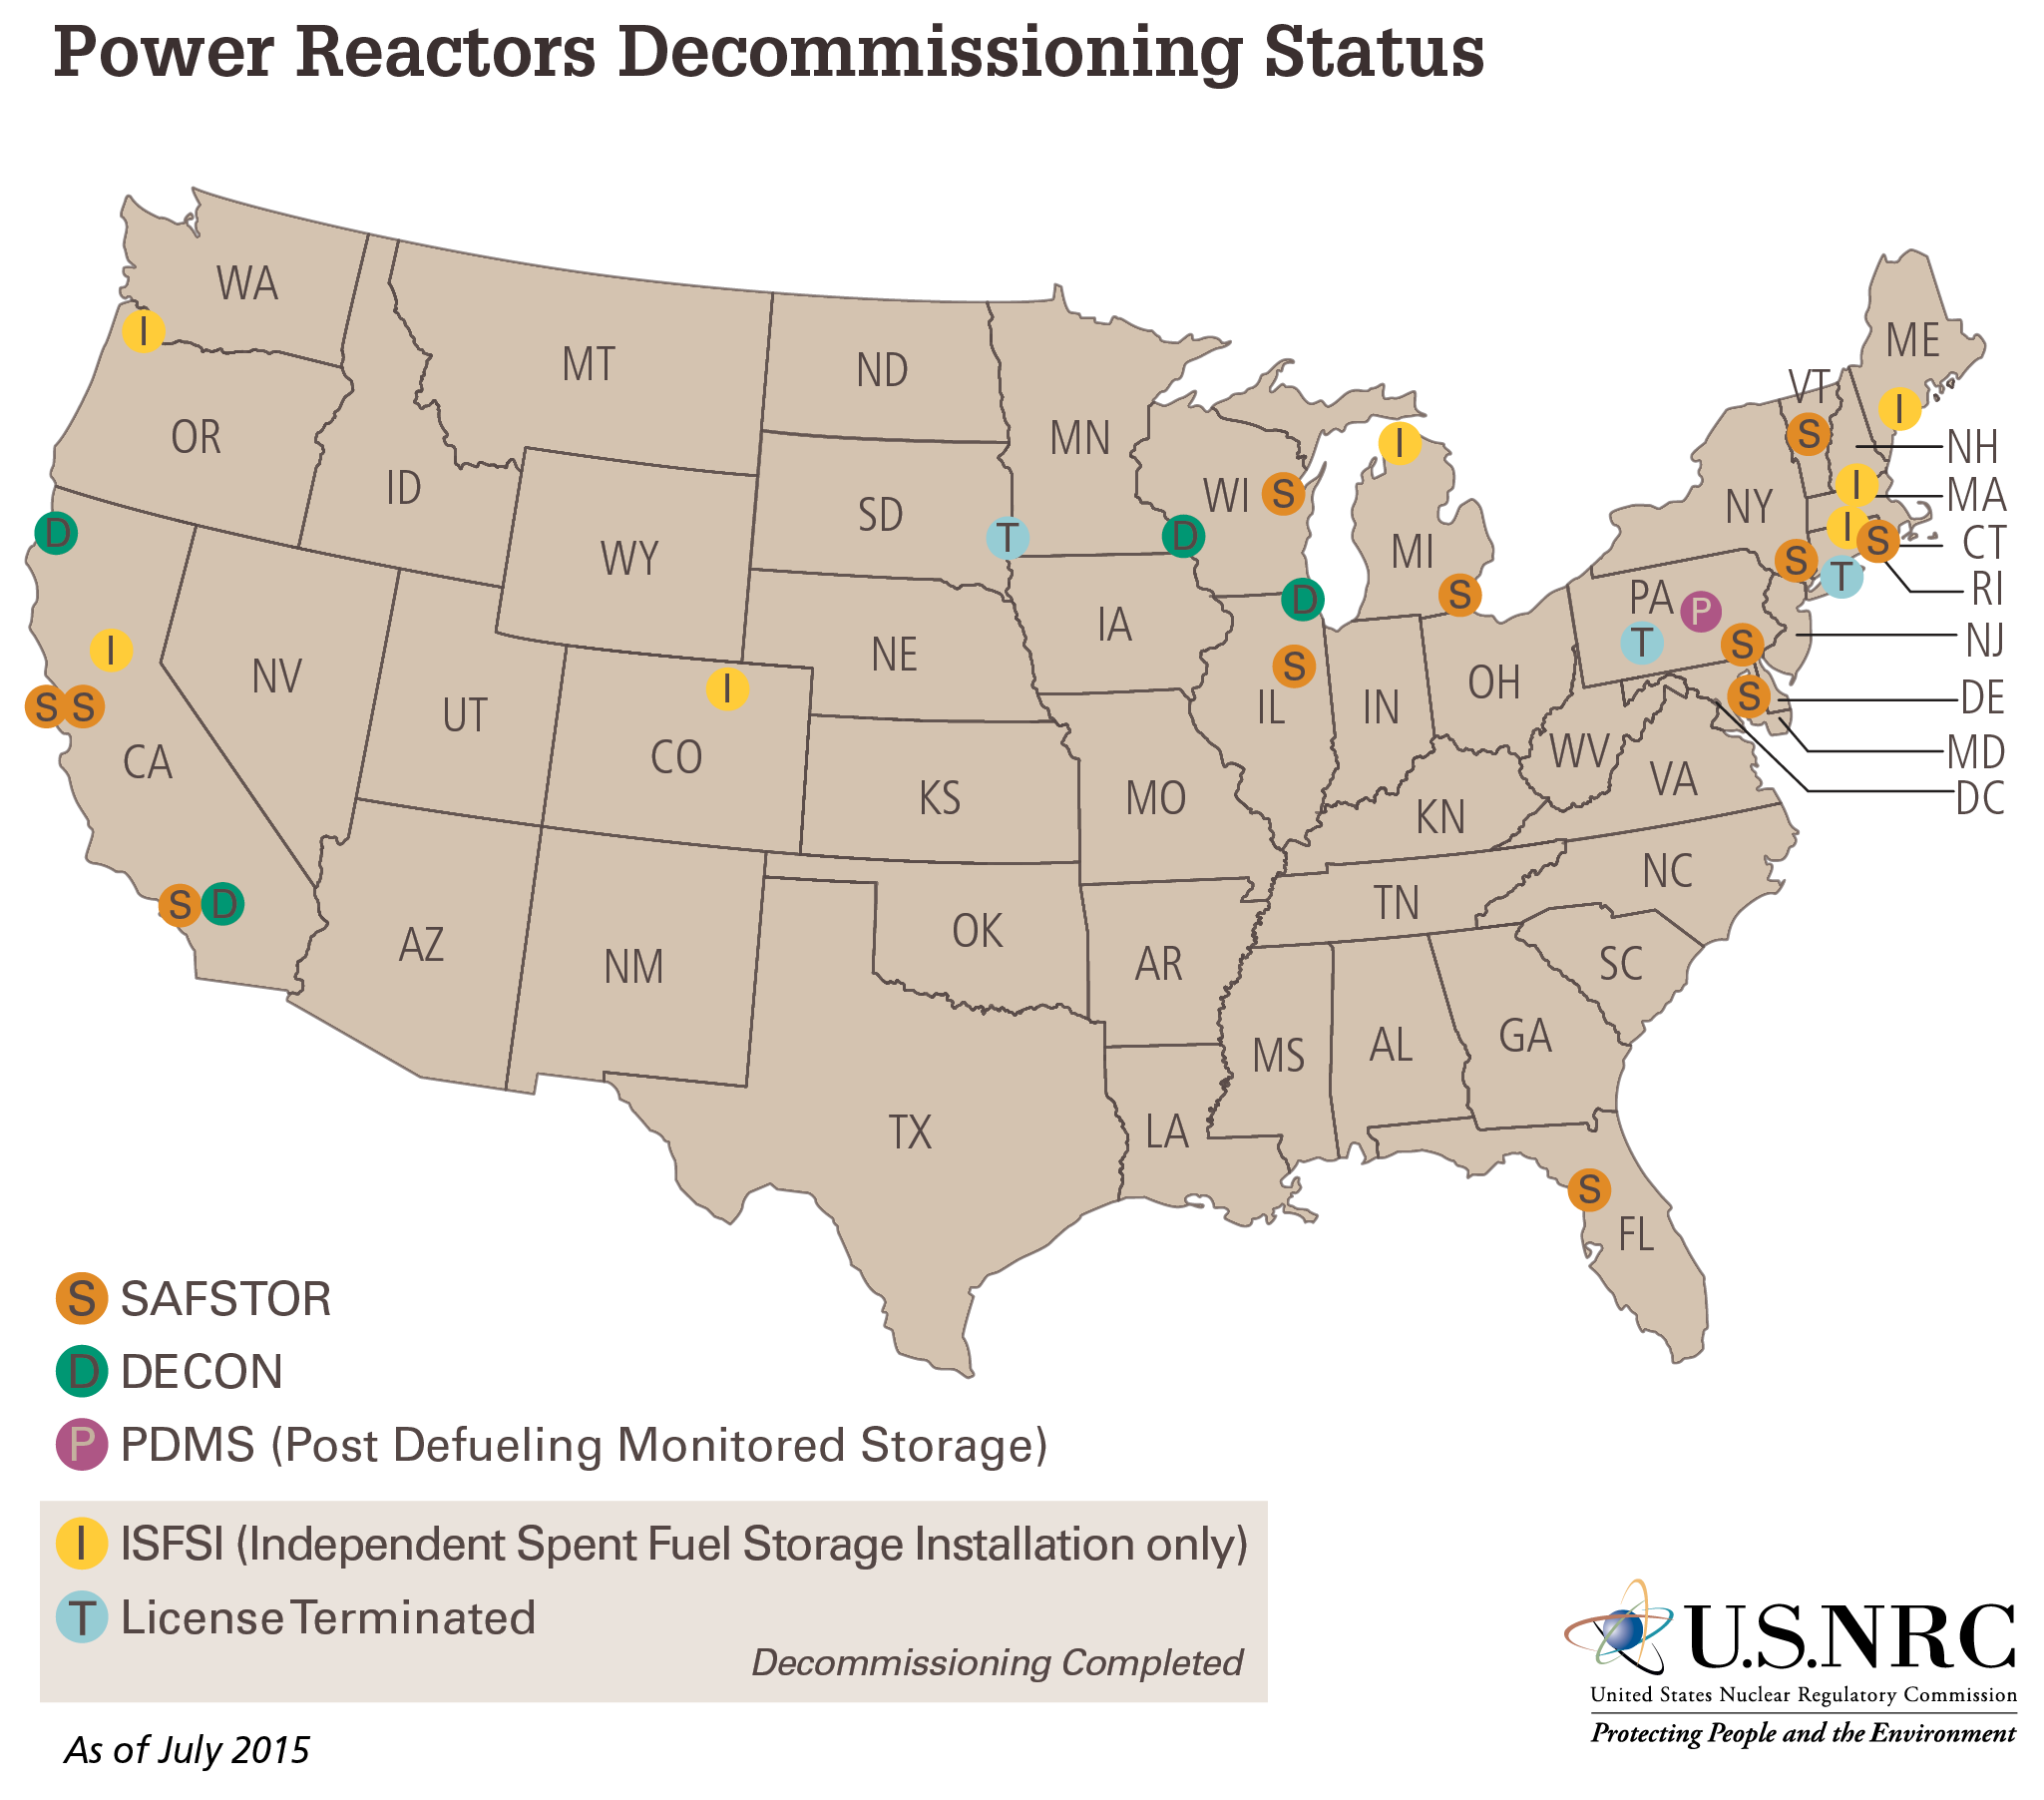
\includegraphics[width=0.8\columnwidth]{power-reactors-decommissioning}	
  \caption{Non-operating facilities status
  \cite{nuclear_regulatory_commission_nrc_2015}.}
  \label{fig:shutdown}
\end{figure}


